% ---------------------------------------------------------------------------
% Investigation 3: Learned Locomotion Control (self-contained draft section)
%
% Written to be pasted into the manuscript as ONE section. Methods, evaluation
% protocol, results, figures, selector, and interpretation are kept together
% so that they can later be distributed across the paper's Methods /
% Experiments / Discussion structure.
%
% Figure files (paths relative to the repository root):
%   PAPER_GRAPHS/figure_1_command_fidelity.pdf
%   PAPER_GRAPHS/rl_section/cot_and_periodicity_seed2.pdf
%   PAPER_GRAPHS/rl_section/push_success_vs_stance_width.pdf
%   PAPER_GRAPHS/rl_section/push_survival_vs_time.pdf
%   PAPER_GRAPHS/high_duty_walk_selector/all_candidate_duty_response_p048.pdf
%   PAPER_GRAPHS/high_duty_walk_selector/combined_fresh_selector_validation_p048.pdf
% Source tables: paper_data/ (see paper_data/MANIFEST.md).
%
% Numbering note: the current manuscript labels the RL study "Investigation 2"
% in the Methods and in the overview table but places it last in the
% Introduction and Abstract. This draft uses "Investigation 3" and the label
% prefix inv3; rename once the order is fixed.
% Citations schulman2017ppo and rudin2022walking are placeholders for the PPO
% and rsl_rl references and are not yet in the bibliography.
% ---------------------------------------------------------------------------

\section{Investigation 3: Learned Locomotion Control}
\label{sec:inv3}

Investigations 1 and 2 relate duty factor to local error convergence and to
constrained-terrain traversal using model-based controllers whose contact
schedule is imposed explicitly. In this investigation we ask whether the same
relationships appear when the locomotion controller is \emph{learned}: a
reinforcement-learning policy is conditioned on the same gait parameters,
and we measure how commanded duty factor, stance width, speed, and gait type
affect (i) whether the requested gait is executed at all, (ii) energetic cost,
and (iii) the ability to keep walking under sustained external pushes. Because
a learned policy has no explicit nominal trajectory or feedback gain, the
saltation-based convergence factor $\chi$ of Sec.~\ref{sec:convergence} cannot
be computed in closed form. We therefore report empirical surrogates and state
explicitly which hypotheses each experiment can and cannot address.

\subsection{Gait-Conditioned Locomotion Policy}
\label{sec:inv3_policy}

\textbf{Task.} We train a proprioceptive locomotion policy for the Unitree Go2
in Isaac Lab using Proximal Policy Optimization (PPO) \cite{schulman2017ppo}
with the \texttt{rsl\_rl} implementation \cite{rudin2022walking}. Conditioning a
locomotion policy on an explicit gait schedule follows prior work that fixes
contact sequences and timings to simplify learning
\cite{yu2026discovery,aractingi2023controlling}; we make no novelty claim for
the formulation itself. The policy acts at 50\,Hz and outputs 12 joint-position
targets, scaled by 0.25 and added to a nominal standing pose, which stock
proportional--derivative controllers ($K_p=25$, $K_d=0.5$) track at 200\,Hz.
The command vector is
\begin{equation}
c_t = [v,\; d,\; w,\; T,\; g],
\end{equation}
where $v$ is forward speed, $d$ the duty factor, $w$ the full left--right foot
separation in the body frame, $T$ the gait period, and $g$ a one-hot gait
identity (two-beat trot or four-beat walk). The gait clock assigns each leg a
phase $\phi_i\in[0,1)$ with the offsets $(0,\tfrac12,\tfrac12,0)$ for trot and
$(0,\tfrac34,\tfrac12,\tfrac14)$ for walk (FL, FR, RL, RR), and a leg is
requested to be in stance while $\phi_i<d$. The 68-dimensional observation
$o_t$ contains body-frame linear and angular velocity, projected gravity, joint
positions and velocities, the previous action, sine and cosine of a
duty-warped phase per leg, the normalized commands and gait one-hot, the four
requested contact flags, the yaw error from the initial heading, and the four
measured foot contacts (foot force above 5\,N). No terrain, map, or beam
information is observed. The actor and critic are multilayer perceptrons with
hidden widths $(256,128,128)$ and ELU activations.

\textbf{Reward.} The per-step reward is
\begin{multline}
r_t = 4\,r_{v} + 8\,r_{\mathrm{contact}} + 8\,r_{w} + 2\,r_{x} + r_{\mathrm{clear}}
      + \tfrac12 r_{h} \\
      - c_{\mathrm{center}} - c_{\mathrm{head}} - c_{\dot\psi},
\label{eq:inv3_reward}
\end{multline}
where $r_v$ rewards tracking the commanded course-frame velocity vector,
$r_{\mathrm{contact}}$ scores agreement between measured foot forces and the
requested stance/swing schedule at every physics substep (duration-balanced so
that a perfectly executed gait scores equally for every $d$), $r_w$ and $r_x$
are Gaussian scores on body-frame lateral and fore--aft foot placement
relative to the commanded stance width and a no-slip stance sweep, $r_{\mathrm{clear}}$
rewards swing-foot clearance, and $r_h$ regulates body height. The bounded costs
penalize lateral drift from the course line, heading error, and body yaw rate.
A fall (base height below 0.16\,m, tilt beyond $60^\circ$, or any non-foot
contact) terminates the episode with a penalty. The reward contains no term
that prefers one duty factor, width, or gait over another.

\textbf{Training distribution.} Commands are resampled every 8--12 gait cycles
from $v\in[0.25,0.40]$\,m/s, $w\in[0.10,0.50]$\,m, $T\in[0.36,0.54]$\,s,
trot at $d\in[0.50,0.75]$, and walk at $d=0.75$, the minimum duty factor of a
four-beat walk without flight phases and the only value shared with trot in
this study. Episodes last up to 20\,s on an open flat plane; 10\,\% of resets
start from a settled four-foot stance. The primary policy (``seed 2'') is
trained from scratch for 1{,}800 PPO updates with 3{,}072 parallel
environments (48-step rollouts, $\gamma=0.995$, $\lambda=0.95$, clip 0.2,
adaptive learning rate) with nominal actuator gains and no external
disturbances. After training, $\theta$ is frozen and only $c_t$ is varied, so
changes in behavior are attributable to the commanded gait parameters.

\textbf{Narrow-stance and push-trained variants.} Two further checkpoints
extend the same policy toward the constrained-terrain setting of
Investigation~2. The \emph{narrow-stance policy} fine-tunes the seed-2 policy
in three successive stages of 1{,}800 updates each, lowering the minimum
sampled stance width to 0.05\,m, tightening the placement reward to a 0.02\,m
scale, feeding the lateral offset from the course line back through the
heading observation, and strengthening the centering cost. These stages also
randomize actuator gains ($0.6$--$1.4\times K_p$, $0.5$--$1.5\times K_d$),
base mass and center of mass, friction, motor strength, joint friction and
armature, and actuator delay (0--20\,ms) at every reset, with the stock Go2
observation noise enabled. The \emph{push-trained policy} continues the
narrow-stance policy for one more stage of 1{,}800 updates with the external
push disturbance of Sec.~\ref{sec:inv3_push} active during training. All
evaluations below use nominal gains and no observation noise unless stated.

\subsection{Evaluation Protocol}
\label{sec:inv3_protocol}

Each evaluated condition uses 64 held-out reset seeds that were never used
during training (32 for the selector grids). A trial starts 0.65\,m behind the
course origin and \emph{succeeds} when the body and all four feet have
traveled 4.0\,m forward without a fall; it \emph{fails} on the fall criteria
above and times out at 20\,s. Because a trial can reach the endpoint while
executing the wrong gait, every trial is also screened for \emph{command
compliance}: over complete gait cycles measured from 200\,Hz foot-force traces,
the achieved duty factor of every leg must be within 0.05 of the command, the
stance-phase foot separation within 0.03\,m of $w$, forward speed within
0.04\,m/s of $v$, stance and swing recall at least 0.90, lateral and heading
root-mean-square error below 0.10\,m and 0.10\,rad, and the sequence of
touchdown and liftoff events must match the commanded gait topology.
Achieved duty factor is the fraction of each cycle for which a foot force
exceeds 5\,N. A condition passes when at least 90\,\% of its trials are
compliant; walking at $d<0.75$ is outside the training support of the seed-2
policy and is reported only to show what the policy does with such commands.

Energetic cost is the positive mechanical cost of transport,
\begin{equation}
\mathrm{CoT}^{+} = \frac{\sum_{k}\sum_{i=1}^{12}\max\!\big(\tau_{k,i}\,\dot q_{k,i},0\big)\,h}{m g \,\Delta x},
\label{eq:inv3_cot}
\end{equation}
sampled at 200\,Hz over four complete cycles after settling, with the applied
joint torque $\tau$, joint velocity $\dot q$, timestep $h=5$\,ms, and forward
displacement $\Delta x$. This omits the resistive-loss term of
Eq.~\eqref{eq:ohmic} because no audited motor-resistance model exists for the
simulated Go2 actuators; $\mathrm{CoT}^{+}$ is therefore used only for
comparisons within this investigation and is not numerically comparable to
the CoT values of Investigation~1. A trial contributes to the energy statistics
only if it is compliant, terminates normally, and makes positive forward
progress.

As a diagnostic for whether the closed-loop gait settles into a period-one
limit cycle, we record whether the contact sequence of the final measured
cycles repeats with the commanded period. This \emph{periodicity} indicator
is a prerequisite for the convergence analysis of Investigation~1, not a
measure of $\chi$. A direct finite-difference estimate of the return-map
Jacobian was also attempted: identical cloned states diverged by 0.016
normalized units within one period because of solver-history effects, the
estimate failed translation-invariance checks at every perturbation radius
tested, and no valid $\chi$ value was obtained. We therefore do not report
$\chi$ for the learned controller.

\subsection{Command Fidelity}
\label{sec:inv3_fidelity}

We first verify that the learned policy realizes the treatment variables. The
seed-2 policy was evaluated at $v=0.30$\,m/s and $T=0.48$\,s over five stance
widths (0.10--0.50\,m), trot at $d\in\{0.50,0.625,0.75\}$, and walk at
$d=0.75$: 20 conditions and 1{,}280 rollouts. All 1{,}280 trials reached the
endpoint and all 20 conditions passed the compliance screen
(Fig.~\ref{fig:inv3_fidelity}). Across condition means, the largest errors
were 0.017\,m in stance width, 0.0007 in duty factor, and 0.012\,m/s in speed,
with lateral and heading errors of at most 0.029\,m and 0.039\,rad RMS. The
policy therefore executes commanded duty factor, stance width, gait type, and
speed independently, including tucked-leg locomotion at a 0.10\,m stance,
which is what allows the remaining experiments to attribute differences to the
commanded parameters.

\begin{figure}[t]
    \centering
    \includegraphics[width=0.48\textwidth]{PAPER_GRAPHS/figure_1_command_fidelity.pdf}
    \caption{Command fidelity of the learned policy at $0.30$\,m/s and
    $T=0.48$\,s (64 held-out rollouts per point). (a)~Achieved body-frame
    stance width and (b)~achieved duty factor follow the commands; (c)~lateral
    and (d)~heading errors stay well inside the compliance limits for all
    gait/duty-factor strata. This validates the experimental inputs; it is not
    a convergence result.}
    \label{fig:inv3_fidelity}
\end{figure}

\subsection{Duty Factor, Periodicity, and Energetic Cost}
\label{sec:inv3_df}

An extended grid with the same seed-2 policy covered four speeds
(0.25--0.40\,m/s), five widths, and both gaits at commanded
$d\in\{0.50,0.625,0.75\}$: 120 conditions and 3{,}840 trials (32 per
condition). Table~\ref{tab:inv3_execution} summarizes execution by gait and
duty factor, and Fig.~\ref{fig:inv3_cot} shows the energetic and periodicity
results.

\begin{table}[t]
    \centering
    \caption{Gait execution of the seed-2 policy over the extended grid
    (640 trials per row, pooled over four speeds and five stance widths).
    Periodic trials settle into a period-one contact sequence; this is a
    diagnostic and not an estimate of $\chi$. Walking below $d=0.75$ lies
    outside the training distribution.}
    \label{tab:inv3_execution}
    \begin{tabular}{llcccc}
        Gait & $d$ cmd. & $d$ achieved & Compliant & Periodic & Falls \\
        \thickhline
        Trot & 0.500 & 0.500 & 591/640 & 356/640 & 0 \\
        Trot & 0.625 & 0.625 & 640/640 & 640/640 & 0 \\
        Trot & 0.750 & 0.750 & 640/640 & 640/640 & 0 \\
        Walk & 0.500 & 0.662 & 0/640   & 161/640 & 1 \\
        Walk & 0.625 & 0.697 & 0/640   & 457/640 & 0 \\
        Walk & 0.750 & 0.750 & 640/640 & 640/640 & 0 \\
    \end{tabular}
\end{table}

\begin{figure}[t]
    \centering
    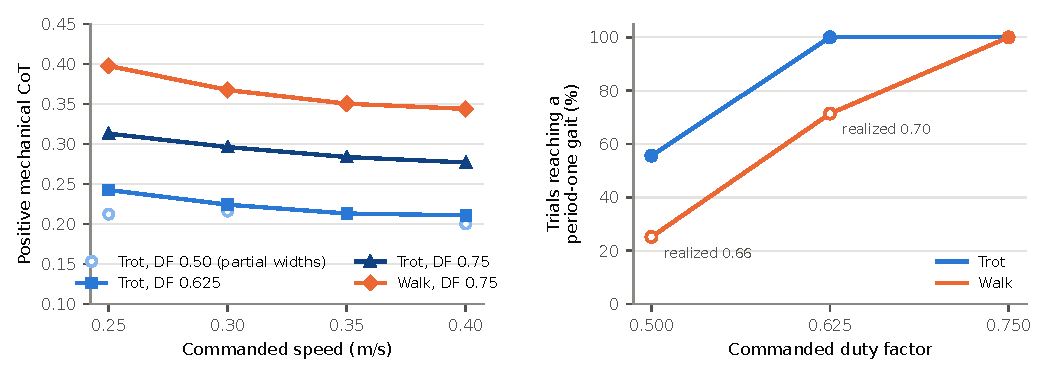
\includegraphics[width=0.48\textwidth]{PAPER_GRAPHS/rl_section/cot_and_periodicity_seed2.pdf}
    \caption{Seed-2 policy on flat ground at $T=0.48$\,s. Left: median positive
    mechanical cost of transport, Eq.~\eqref{eq:inv3_cot}, over the five stance
    widths; open markers pool only the widths whose trials passed the energy
    validity gate (trot at $d=0.50$ never passed at all five widths). Right:
    fraction of trials whose contact sequence settles to a period-one gait,
    pooled over speeds and widths; open markers denote non-compliant
    conditions and are labeled with the duty factor the policy actually
    produced.}
    \label{fig:inv3_cot}
\end{figure}

Three observations follow. First, the low-duty-factor trot is the only
in-distribution stratum with degraded execution: 49 of 640 trials failed the
compliance screen and only 56\,\% settled to a period-one gait, against
100\,\% for trot at $d\geq0.625$ and for walk at $d=0.75$. The non-periodic
low-duty trials are not falls; their contact sequence simply does not repeat
with the commanded period within the measured cycles, so they never reach the
steady gait that a convergence analysis presupposes. Second, the learned
four-beat walk does not exist below $d=0.75$: commanded walks at $d=0.50$ and
$0.625$ were executed at $d\approx0.66$ and $0.70$ with the wrong contact
topology, and the only fall in the 3{,}840 trials occurred in this regime.
The learned policy thus respects the same lower bound on walking duty factor
that the trajectory optimizer in Investigation~1 imposes by construction.
Third, energetic cost rises with duty factor for trot
($\mathrm{CoT}^{+}\approx0.21$--$0.24$ at $d=0.625$ versus $0.28$--$0.31$ at
$d=0.75$), decreases mildly with speed over the narrow 0.25--0.40\,m/s range
for every stratum, and is higher for walk than for trot at the matched
$d=0.75$ ($0.34$--$0.40$). Widening the stance from 0.10 to 0.50\,m raised
$\mathrm{CoT}^{+}$ in every stratum, by 4--10\,\% for trot at $d=0.75$,
17--22\,\% for trot at $d=0.625$, and 40--48\,\% for walk, so the narrow
stances that are hardest to stabilize are also the cheapest to execute.
Because energy validity is factor-dependent (all cells valid at $d\ge0.625$,
only 5 of 20 cells valid for trot at $d=0.50$), we do not fit correlations
across the whole grid.

\subsection{Robustness to External Pushes at Narrow Stance}
\label{sec:inv3_push}

To test whether duty factor and stance width predict robustness of the learned
controller, we apply a sustained random disturbance to the base during flat
ground trials and count the trials that still complete the 4\,m course. The
disturbance is a piecewise-constant world-frame wrench on the base link:
every 0.1--0.4\,s a new direction (uniform in the horizontal plane with a
vertical component of at most 25\,\%) and a magnitude fraction uniform in
$[0,1]$ are drawn. The magnitude bound ramps linearly from 10\,\% to 100\,\% of
25\,N and 3\,N\,m over the first 10\,s of each trial, so every trial begins
lightly disturbed and is pushed harder the further it goes. The same
disturbance sequence is replayed for every condition. This protocol stresses
recovery from repeated, growing pushes during locomotion; it is not the
impulse-response experiment of Investigation~1 and does not estimate
$\chi$.

We evaluate the narrow-stance policy (trained without pushes) and the
push-trained policy under identical nominal and pushed conditions: trot at
commanded $d\in\{0.50,0.625,0.75\}$ and commanded stance widths
$w\in\{0.05,0.06,0.08,0.10\}$\,m, at 0.30\,m/s and $T=0.48$\,s, 64 trials per
condition (768 per policy and disturbance level). Two properties of these
checkpoints must be stated before interpreting the results, because they are
measured from the same archives (Table~\ref{tab:inv3_push}). (i)~The
fine-tuned checkpoints no longer realize the commanded duty factor exactly:
without pushes they execute $d\approx0.67$, $0.72$, and $0.78$ for commands
$0.50$, $0.625$, and $0.75$, so the duty-factor contrast available here is
compressed to the realized range 0.67--0.78. All contrasts below are stated
on realized values. (ii)~The narrow-stance policy realizes the commanded
stance width (0.056--0.098\,m), whereas the push-trained policy widens its
stance to 0.13--0.18\,m regardless of command. The push-trained policy
therefore cannot be used to test the stance-width hypothesis at narrow
widths, and its results are reported as a second, wider-stance data set.

\begin{table}[t]
    \centering
    \caption{Push study: trials completing 4\,m under the ramped disturbance,
    out of 64 per cell, at 0.30\,m/s and $T=0.48$\,s. Without pushes every
    cell scored 64/64 for both policies. $\bar d$ and $\bar w$ are the duty
    factor and stance width realized by each policy in the undisturbed trials,
    pooled over the other factor.}
    \label{tab:inv3_push}
    \begin{tabular}{lcccc|cccc}
        & \multicolumn{4}{c|}{Narrow-stance policy} & \multicolumn{4}{c}{Push-trained policy} \\
        $w$ cmd. (m) & 0.05 & 0.06 & 0.08 & 0.10 & 0.05 & 0.06 & 0.08 & 0.10 \\
        $\bar w$ (m) & 0.056 & 0.064 & 0.080 & 0.098 & 0.139 & 0.145 & 0.156 & 0.168 \\
        \thickhline
        $d=0.50$ cmd. ($\bar d=0.67$, $0.66$)  & 3  & 5  & 14 & 18 & 51 & 56 & 53 & 58 \\
        $d=0.625$ cmd. ($\bar d=0.72$, $0.72$) & 11 & 11 & 28 & 43 & 59 & 61 & 61 & 63 \\
        $d=0.75$ cmd. ($\bar d=0.78$, $0.77$)  & 5  & 19 & 24 & 42 & 62 & 63 & 63 & 63 \\
        \hline
        All & 19 & 35 & 66 & 103 & 172 & 180 & 177 & 184 \\
    \end{tabular}
\end{table}

\begin{figure*}[t]
    \centering
    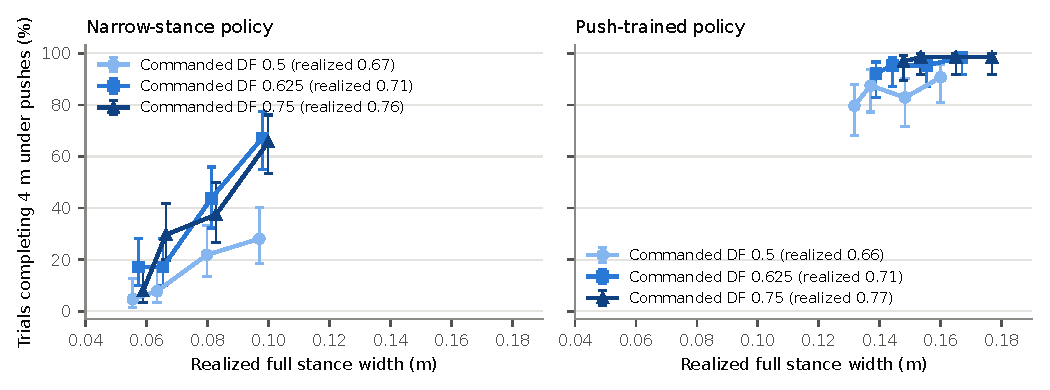
\includegraphics[width=0.98\textwidth]{PAPER_GRAPHS/rl_section/push_success_vs_stance_width.pdf}
    \caption{Fraction of trials completing the 4\,m course under the ramped
    push disturbance, plotted against the stance width each policy actually
    realized (64 trials per point, Wilson 95\,\% intervals). Left: the
    narrow-stance policy tracks the commanded width; success rises steeply
    with stance width and is lowest for the lowest realized duty factor.
    Right: the push-trained policy survives 93\,\% of trials but does so
    while widening its stance to 0.13--0.18\,m, so its points do not test
    narrow-stance locomotion; within it, success still increases
    monotonically with realized duty factor. Realized duty factors in the
    legends are measured during the pushed trials and are 0.01--0.02 below
    the undisturbed values in Table~\ref{tab:inv3_push}.}
    \label{fig:inv3_push}
\end{figure*}

\begin{figure}[t]
    \centering
    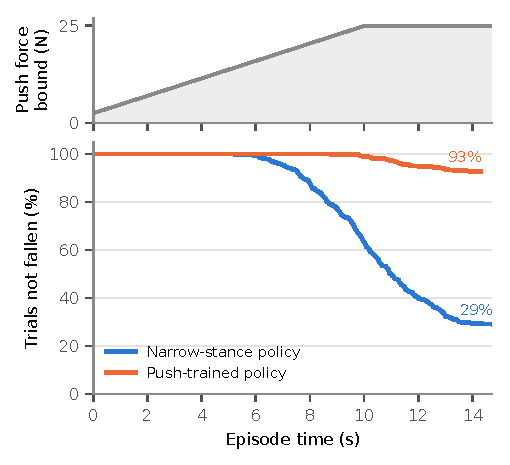
\includegraphics[width=0.44\textwidth]{PAPER_GRAPHS/rl_section/push_survival_vs_time.pdf}
    \caption{Survival of all 768 pushed trials per policy against episode
    time, with the push-force bound of the disturbance schedule. Falls of the
    narrow-stance policy begin near 6\,s, when the bound reaches about
    15\,N, and accelerate as the bound saturates at 25\,N; the push-trained
    policy loses trials only after the bound saturates.}
    \label{fig:inv3_survival}
\end{figure}

Without pushes, both policies completed all 768 trials in every cell. Under
pushes the narrow-stance policy completed 223 of 768 trials (29\,\%), and the
push-trained policy 713 of 768 (93\,\%). For the narrow-stance policy, success
pooled over duty factor rose monotonically with realized stance width, from
10\,\% at 0.056\,m to 18\,\%, 34\,\%, and 54\,\% at 0.064, 0.080, and
0.098\,m (Fig.~\ref{fig:inv3_push}, left). Pooled over width, success was
16\,\% at realized $d=0.67$ and 36\,\% at $d=0.72$, but did not increase
further at $d=0.78$ (35\,\%); the confidence intervals of the 0.72 and 0.78
conditions overlap at every width. Mean time to failure also increased with
both width and realized duty factor (8.6\,s at $w=0.05$\,m, $d=0.67$ versus
11.7\,s at $w=0.10$\,m, $d=0.78$). Fig.~\ref{fig:inv3_survival} shows that
the narrow-stance policy begins to fall once the push bound reaches roughly
15\,N, whereas the push-trained policy begins to lose trials only after the
bound saturates at 25\,N. For the push-trained policy, success rose
monotonically with realized duty factor at every stance width (85\,\%,
95\,\%, and 98\,\% pooled over width for $d=0.66$, $0.72$, and $0.77$), while
its realized width varied too little (0.13--0.18\,m) and too far from the
commands to support a width contrast.

The push-trained policy's widening of its stance is itself informative. Its
training reward penalizes placement error with a 0.02\,m scale, so a stance
0.08\,m wider than commanded forfeits nearly the entire placement reward;
the policy nevertheless converged to that stance because survival under pushes
was worth more. A learned controller that is free to choose therefore gave up
narrow stance to gain robustness, which is the direction predicted by
hypothesis~3, but it also shows that the width command was not honored, so the
push-trained result cannot be read as robust \emph{narrow} locomotion.

\subsection{Automatic Duty-Factor Selection}
\label{sec:inv3_selector}

Investigation~2 selects duty factor by hand for each terrain width. Here we
ask whether a duty factor can instead be selected automatically from the
locomotion context, and what such a selector chooses as the stance narrows.
The selector is a separate module: gait type, speed, period, and stance width
remain specified, and the selector outputs only $d$, which is then passed to
the fixed locomotion policy. Two selector experiments were run, each with its
own separately trained low-level policy; they are not interchangeable and are
reported as two controllers.

\textbf{Selection rule.} For every context
$(w, v, T, g)$ and every candidate duty factor $d_j$, 32 held-out trials are
run with the low-level policy, settling for 8 cycles (12 for the walking
controller) and measuring the final 4. A candidate is \emph{eligible} if at
least 90\,\% of its trials are compliant with finite $\mathrm{CoT}^{+}$. The
label for the context is the eligible candidate with the lowest median
$\mathrm{CoT}^{+}$,
\begin{equation}
d^{\star}(w,v,T,g) = \operatorname*{arg\,min}_{d_j \in \mathcal{E}(w,v,T,g)}\;
\operatorname{median}\,\mathrm{CoT}^{+}(d_j),
\label{eq:inv3_selector}
\end{equation}
where $\mathcal{E}$ is the eligible set; contexts with no eligible candidate
receive no label. A small feedforward network (two hidden layers of 32 ELU
units) is fitted from the context to $d^\star$ with its output bounded to the
feasible duty-factor range, and the fitted selector is then validated in 32
fresh trials per context, requiring at least 90\,\% compliance and a median
achieved duty factor within 0.05 of the selection. Because the criterion is
energetic, the selector picks the \emph{cheapest gait that the policy can
still execute reliably}; robustness enters only through the eligibility gate,
not through any disturbance test. Selector choices are therefore evidence
about the feasible operating range of the learned controller, not direct
evidence of improved robustness.

\textbf{Adaptive controller (seed 3).} A low-level policy was trained with
both gaits balanced over candidate $d\in\{0.50,0.55,\dots,0.75\}$ and
evaluated at $T=0.48$\,s over $w\in\{0.10,\dots,0.50\}$\,m and
$v\in\{0.25,\dots,0.40\}$\,m/s (10{,}240 grid trials).
Fig.~\ref{fig:inv3_candidates} shows every measured candidate. For trot, the
two lowest candidates ($d=0.50$ and $0.55$) failed compliance at the narrow
widths (0.10 and 0.20\,m) but $d=0.55$ passed at 0.30\,m and wider, so the
selector chose $d^\star=0.65$ at $w=0.10$\,m and $0.25$\,m/s, $0.60$ at
$0.10$--$0.20$\,m, and $0.55$ at $0.30$--$0.40$\,m (realized 0.667, 0.625,
and 0.583 after the 24-tick period quantization). At $w=0.50$\,m the selection
rose again to $0.60$ at some speeds, so the width relationship is not
globally monotonic. For walk, no candidate below $d=0.75$ was ever compliant,
so the selector chose $d^\star=0.75$ in every context. All 40 selected
contexts (20 trot, 20 walk) passed fresh validation with 32/32 compliant
trials (Fig.~\ref{fig:inv3_selector_validation}).

\textbf{High-duty walking controller (seed 4).} Because the adaptive
controller's walk was pinned at its lower feasibility bound, a second policy
was trained for walk only with candidates $d\in\{0.75,0.80,0.85,0.90\}$ at
$T=0.48$\,s. Over the same 20 width--speed contexts, $d=0.80$ was eligible in
all 20, $d=0.85$ in 3, and $d=0.75$ and $0.90$ in none, so the selector chose
$d^\star=0.80$ everywhere (realized median $0.823$ because a 24-tick period
quantizes the schedule) and every context passed fresh validation with 32/32
compliant trials. This controller showed no dependence of the selected duty
factor on stance width or speed within the tested domain.

\begin{figure*}[t]
    \centering
    \includegraphics[width=0.98\textwidth]{PAPER_GRAPHS/high_duty_walk_selector/all_candidate_duty_response_p048.pdf}
    \caption{All measured duty-factor candidates for the adaptive controller
    (trot, top; walk, bottom, solid) and the high-duty walking controller
    (walk, dashed) at $T=0.48$\,s, by commanded speed. Colored curves are the
    achieved duty factor across stance width, crosses mark candidates that
    failed the 90\,\% compliance gate, and black curves are the validated
    selector outputs. Low-duty trot becomes non-compliant as the stance
    narrows, which drives the selected duty factor upward at 0.10--0.20\,m.}
    \label{fig:inv3_candidates}
\end{figure*}

\begin{figure}[t]
    \centering
    \includegraphics[width=0.48\textwidth]{PAPER_GRAPHS/high_duty_walk_selector/combined_fresh_selector_validation_p048.pdf}
    \caption{Duty factor realized in fresh validation of the fitted selectors
    at $T=0.48$\,s. Filled markers: adaptive controller (seed 3); open markers:
    high-duty walking controller (seed 4). Trot selects a higher duty factor at
    narrow stance widths; the learned walks are executable only at
    $d\geq0.75$ and select a constant value.}
    \label{fig:inv3_selector_validation}
\end{figure}

\subsection{Relationship to the Hypotheses}
\label{sec:inv3_hypotheses}

The learned-controller experiments provide partial evidence and several
explicit limitations, summarized against the four hypotheses.

\textbf{H1 (speed worsens convergence).} Not tested. No convergence measure
was obtained for the learned controller, and the push study was run at a
single speed. Over the narrow trained range of 0.25--0.40\,m/s, execution,
periodicity, and compliance were unaffected by speed, and $\mathrm{CoT}^{+}$
decreased mildly with speed in every stratum; this range is far below the
speeds at which Investigation~1 found any speed effect.

\textbf{H2 (higher duty factor improves convergence).} Directionally
supported, with qualifications. Low-duty trot ($d=0.50$) was the only
in-distribution gait that failed to settle to a period-one cycle in a large
fraction of trials, and under sustained pushes success increased from a
realized $d=0.67$ to $0.72$ for the narrow-stance policy and monotonically
from $0.66$ to $0.77$ for the push-trained policy. Two caveats apply: the
fine-tuned checkpoints compressed the realized duty-factor range to
0.66--0.78, so the low-duty regime where Investigation~1 predicts the largest
effect was not reached in the push study, and the narrow-stance policy did not
improve further above $d\approx0.72$. The energetic cost of a higher duty
factor was also clearly measurable ($\mathrm{CoT}^{+}$ about 30\,\% higher
at $d=0.75$ than at $0.625$ for trot), so the learned controller exhibits the
same robustness--efficiency trade-off that motivates selecting the smallest
adequate duty factor.

\textbf{H3 (narrower stance worsens convergence).} Supported in the sense
available here. With the stance width honored (narrow-stance policy), push
survival fell from 54\,\% at a realized 0.098\,m to 10\,\% at 0.056\,m, and
the energy-based selector raised the trot duty factor as the commanded width
decreased from 0.30 to 0.10\,m because low-duty trot stopped being
executable. When freed to trade placement reward for survival, the
push-trained policy widened its stance. All of these are flat-ground
experiments with a commanded foot separation; none imposes the physical
support constraint of a beam, so they show sensitivity to lateral stance
margin rather than beam traversal.

\textbf{H4 (walking is more convergent than trotting).} Not established.
At the matched $d=0.75$ the learned walk and trot were indistinguishable in
command fidelity and periodicity (both 100\,\%), and walk was less efficient,
consistent with Investigation~1's finding that gait type is a weak predictor
once duty factor is matched. The push study included trot only, and no
convergence measure exists for either gait. What the learned controller does
show is that the two gaits have different feasible duty-factor ranges: trot
was executable from $d=0.50$ upward, while the four-beat walk was never
executed correctly below $d=0.75$ and, for the high-duty controller, preferred
$d\approx0.82$. In a learned controller, gait type therefore constrains which
duty factors are available rather than determining robustness at a given duty
factor.

\textbf{Limitations.} Each result comes from a single trained policy per
controller variant, so it is descriptive rather than a population-level
replication; the compliance-gated energy statistics have factor-dependent
missingness at low duty factor; the fine-tuned checkpoints used in the push
study track duty factor and (for the push-trained policy) stance width less
accurately than the seed-2 policy; and no closed-loop $\chi$ was measured.
Establishing the convergence hypotheses for learned control would require
either a numerically reliable return-map estimator or matched impulse-response
experiments across independently trained policies, and testing the beam
hypothesis would require restoring a physical support constraint in the
evaluation environment.
